\chapter{Calibration}
\label{ch:calibration}

\section{\pmt}
\label{sec:pmt}

Pulseheight/integral
Number of particles, leptons and gammas, separate?


\subsection{LED calibration}
\label{sub:led_calibration}

Setup where we can use an optical fiber pointed at the windows of the
\pmt to send bursts of photons at the \pmt. Similar to a pulse
generator, but with light. Not much control over the intensity and
during of the pulse, but pulses are short (\SI{20}{\nano\second}) and
have a reasonable strength and width, making them comparable to real
signals. Signal strength fluctuations..
Intensity?

Using multiple fibers for one \pmt to increase signal strength...
Checking linearity of light input versus signal from \pmt.


\section{\gps accuracy}
\label{sec:gps_accuracy}

This described time difference calibration measurements performed on
HiSPARC II and III electronic boxes. This started after Dr. David
Fokkema discovered an unexpected time offset between timestamps of
events in a test where two HiSPARC stations (501 and 502) were triggered
with the same pulse generator. Since these stations are very close
($\sim\SI{100}{\meter}$) a minimal time offset was expected, any offset
or large standard deviation was expected to be the result of errors in
\gps accuracy and position. However, a large offset ($\Delta t
\sim\SI{18}{\nano\second}$) was found. Further tests with other \hisparc
electronics and various setups were performed. Both the \hisparc
electronics and \gps antennas were found to have varying offsets
contributing to time differences in the resulting time measurements. The
offsets in the \hisparc electronics can be as high as $|\Delta t| =
\SI{50}{\nano\second}$ and in the \gps $|\Delta t| \approx
\SI{8}{\nano\second}$ [not a lot of samples]. While the $\sigma_{\Delta
t}$ remains within GPS specifications ($\sigma_{\Delta t} <
\SI{4.5}{\nano\second}$).


\subsection{Making timestamps}
\label{sub:gps_timestamps}

%\citep{Verkooijen:2008tq}
In the report Message Structures \hisparc the method used for
determining the time for an event is thoroughly explained. Every second
the \gps receiver sends a signal (a Pulse Per Second) to the \hisparc
electronics. The \hisparc box uses a $\SI{200}{\mega\hertz}$ clock to
determine the time within this second. Since the crystal in this clock
does not work at exactly $\SI{200}{\mega\hertz}$ the counter (reset at
the arrival of a PPS) is read at the moment of an event and then when
the next PPS arrives. Giving information about at what fraction of that
second the event occured. For higher accuracy (more than
$\SI{5}{\nano\second}$) the clock is also read on the negative side of
the clock, making the system clock an effective
$\SI{400}{\mega\hertz}$ clock.

$Event time = E_{Sync} + E_{Quan1} + (\frac{T_{Event}}{T_{PPS}}) (1e^9 -
E_{Quan1} + E_{Quan2})$

Where $E_{Quan}$ is the Quantization Error, $E_{Sync}$ is the
Synchronization Error, $T_{Event}$ are the count of ticks till the event
and $T_{PPS}$ are the count of ticks between the PPS before and after
the event.

FIX - Explain 3 one second messages are needed to make timestamp.
Messages Structures HiSPARC p.2


\subsection{Test setup}
\label{sub:gps_test_setup}

In the setup one \hisparc II Master (hardware serial: 62) is used as the
main reference point for the entire test. All other \hisparc boxes were
tested against this reference one at a time to measure the offset. Two
\gps antennas ('501' and 'test') and a \gps splitter were used. With
these it was possible to perform tests in which both \hisparc boxes used
the same \gps antenna, removing the offset caused by using different
\gps antennas.

Each \hisparc box was connected to a \gps antenna and a PC, each running
the current version of the \hisparc Software; \hisparc DAQ II v3.0.4.
When the \hisparc III boxes needed to be tested the DAQ was upgraded to
the beta version of the new DAQ; \hisparc DAQ III v1.0.0.

A 100Mhz Pulse Generator (as reference: Tabor Electronics Model 8600),
with two short equal-length signal cables and a signal splitter was used
to trigger the \hisparc electronics. Each box was connected to the same
pulse generator through either of the PMT input channels. To ensure the
generated signals arrived at the same time at the input both cables from
the pulse generator were connected to the same \hisparc electronics and
also switched around.

\begin{figure}
    \centering
     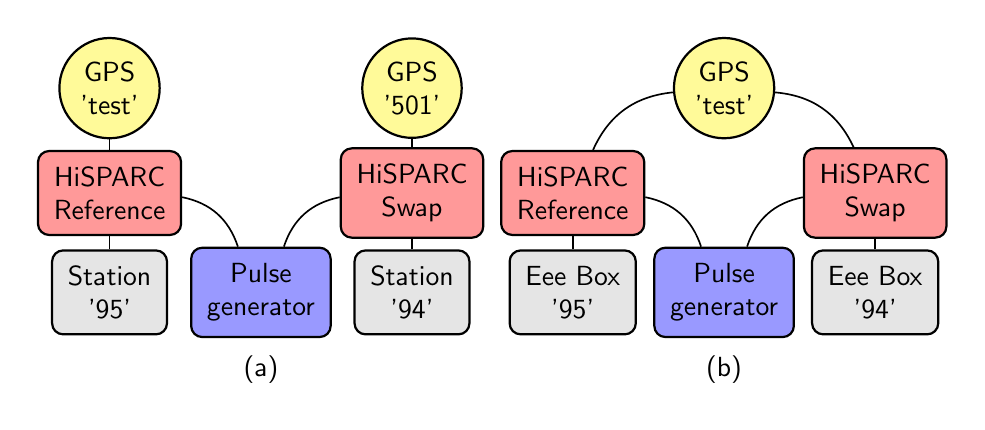
\begin{tikzpicture}
  [font=\sffamily,
   every matrix/.style={ampersand replacement=\&,column sep=0.1cm,row sep=0.1cm},
   gps/.style={draw,thick,circle,fill=yellow!40,inner sep=.1cm, align=center},
   pc/.style={draw,thick,rounded corners,fill=black!10,inner sep=.2cm, align=center},
   hisparc/.style={draw,thick,rounded corners,fill=red!40,inner sep=.2cm, align=center},
   pulse/.style={draw,thick,rounded corners,fill=blue!40,inner sep=.2cm, align=center},
   to/.style={-,semithick,font=\sffamily\footnotesize},]

  \matrix{
   \node[gps] (test) {GPS\\'test'}; \& \& \node[gps] (501) {GPS\\'501'}; \& \& \& \node[gps] (b_test) {GPS\\'test'}; \& \\
   \node[hisparc] (refr) {HiSPARC\\Reference}; \& \& \node[hisparc] (swap) {HiSPARC\\Swap}; \& \& \node[hisparc] (b_refr) {HiSPARC\\Reference}; \& \& \node[hisparc] (b_swap) {HiSPARC\\Swap}; \\
   \node[pc] (95) {Station\\'95'}; \& \node[pulse] (pulse) {Pulse\\generator}; \& \node[pc] (94) {Station\\'94'}; \& \& \node[pc] (b_95) {Eee Box\\'95'};  \& \node[pulse] (b_pulse) {Pulse\\generator}; \& \node[pc] (b_94) {Eee Box\\'94'}; \\
   \& \node {(a)}; \& \& \& \& \node {(b)}; \& \\
  };
  
  \draw[to] (test) -- node[below,above,sloped] {} (refr);
  \draw[to] (501) -- node[below,above,sloped] {} (swap);
  \draw[to] (95) -- node[midway,midway,sloped] {} (refr);
  \draw[to] (94) -- node[midway,midway,sloped] {} (swap);
  \draw[to] (pulse) to[bend left] node[above,below,sloped] {} (swap);
  \draw[to] (pulse) to[bend right] node[above,below,sloped] {} (refr);

  \draw[to] (b_test) to[bend right] node[below,above,sloped] {} (b_refr);
  \draw[to] (b_test) to[bend left] node[below,above,sloped] {} (b_swap);
  \draw[to] (b_95) -- node[midway,midway,sloped] {} (b_refr);
  \draw[to] (b_94) -- node[midway,midway,sloped] {} (b_swap);
  \draw[to] (b_pulse) to[bend left] node[above,below,sloped] {} (b_swap);
  \draw[to] (b_pulse) to[bend right] node[above,below,sloped] {} (b_refr);

 \end{tikzpicture}

    \caption{This image shows the setup of the test, two PCs (Eee Box)
             with HiSPARC Masters (Reference and Swap), both connected
             to the same pulse generator. Each is also connected to a
             \gps, some tests used separate \gps antennas (a) and in
             some tests the same \gps was used by both (b).}
    \label{fig:setup}
\end{figure}


\subsection{Calibration}
\label{sub:gps_calibration}

[tijdtest]
One reference, compared to another \hisparc electronics box.
Each connected to a/same gps, triggered by same pulse generator.
\gps timestamps compared.


\subsection{Offsets between \hisparc electronics}
\label{sub:gps_offsets}

Found different offsets between each \hisparc electronics unit.
Constant over time. Can be corrected.

Importance of 24 hour self-survey.

Tested again year later, same difference??

['box-plot' like image showing the mean offsets and errors]
